\documentclass[main.tex]{subfiles}

\begin{document}
\chapter{Nuclear physics}

\section{Introduction}

Things to remember about nuclear units: \(\hbar c \approx \SI{197}{MeV fm} \) and \(\SI{}{MeV fm} = \SI{10}{eV \angstrom} \); there are weird things like \(e^2 = \SI{1.44}{MeV fm} \), \(4 \pi \varepsilon_0 = \). The atomic mass unit is equal to \(\SI{931.5}{MeV} \).

We have indetermination both between position and momentum: \(\Delta x \Delta p \geq \hbar/2\) and between time and energy: \(\Delta E \Delta t \geq \hbar /2\).

We can characterize the atomic particles by mass \(m\), charge \(q\), spin \(s\), half-life and mean charge radius \(\expval{\rho r^2} \sqrt{c} \): this last quantity is of the order \(\SI{.87}{fm}\) for the proton, and \(\SI{-0.1}{fm} \) for the neutron.

\section{Nuclear density}

It it roughly constant up to some radius, then it decays.
The proper way to write it would be to sum the modulus square of the wavefunction \(\psi_i\) of every nucleon:

\begin{equation}
    \rho(r) = \sum _{i} \abs{\psi_i (r)}^2
\end{equation}

We can approximate it as a radial distribution

\begin{equation}
    \rho(r) \sim \frac{\rho_0}{1 + \exp(\frac{r - r_0}{a})}
\end{equation}

where \(\rho_0 \approx 0.15 \divisionsymbol \SI{0.2}{ nucleons  \per fm^3} \) is the approximately constant density in the central region, \(r_0 \approx 1.20 \divisionsymbol \SI{1.25}{fm} A ^{1/3}  \) is the approximate radius of the nucleus (corresponding to where the density becomes half of \(\rho_0\)), \(a \approx 0.65 \divisionsymbol \SI{0.7}{fm} \) is the \emph{diffusivity}, which quantifies the length scale at which the density distribution goes to zero.

\begin{bluebox}
  Taking \(r_0 \approx \SI{1.2}{fm} \), we can estimate the nucleon density

  \begin{equation}
      \rho_0 \approx \frac{A}{V} = \frac{A}{\frac{4}{3} \pi \qty(r_0 A^{1/3})^3} \approx \SI{0.138}{fm^{-3}}
  \end{equation}

  and the corresponding mass density will be \(\approx \SI{129}{MeV \per fm^3}\) corresponding to \( \SI{2.3e17}{kg \per m^3}\), which is huge when compared to, say, that of a block of Osmium, which is around \(\SI{2.26e5}{kg \per m^3}\).
\end{bluebox}

There are also asymmetric effects, such as a skin of neutrons in the outermost part of the nucleus or a halo, which extends much further than a skin. This can be seen by looking at the differences in the scattering cross section \(\sigma \approx \pi r_0^2\).

We distinguish the nuclei by the proton number \(Z\), the neutron number \(N\) and their sum \(A = N+Z\). They are written as \(^{A} [Z]\).

\begin{itemize}
    \item Isotopes have the same \(Z\), \(^{235} \ce{U} \) and \(^{233} \ce{U}  \);
    \item Isobares have the same \(A\), \(^{44} \ce{Ca} \) and \(^{44} \ce{Ti} \);
    \item Isotones have the same \(N\), \(^{40} \ce{Ca} \) and \(^{38} \ce{Ar} \);
    \item Isomeres have the same \(Z\) and \(N\), but are in different excitation states. We require them to be somewhat stable, with half-life \({\gtrsim \SI{e-12}{s}}\), \(^{99}\ce{Tc}  \) and \(^{99m}\ce{Tc}  \).
\end{itemize}

We also define specular nuclei: denoting the nuclear numbers as \((N,Z)\), \((a, b)\) is isobaric and specular to \((b, a)\).

\begin{bluebox}
  At the driplines, the excess nucleons are not bound (the effective potential they are in does not have a minimum).

  \(^{8} \ce{B} \) and \(^{8} \ce{Be} \) are isobares.

  \(^{19} \ce{F} \) is an isotone to \(^{17} \ce{F} \).

  The stable isotopes of Samarium are those with \(A=144\), 150, 152, 154.

  The specular nuclide to \(^{11} \ce{Li} \) would be \(^{11} \ce{O} \), but it does not seem to exist.
\end{bluebox}

The mass of a nuclide is given by

\begin{equation}
M (A, Z) = Z m_p + (A-Z) m_n - B(A, Z)
\end{equation}

 where \(B\) is the binding energy. It is a good first approximation to say \(B/A \approx \text{const}\), around \(\SI{8}{MeV} \).

Actually, this value increases up to iron, then very slowly decreases, with slight bumps at magic numbers.

\section{Waterdrop model}

A nucleus is similar to a water droplet, like:

\begin{itemize}
    \item \(\nabla \cdot \vec{v} = 0  \) and similarly the nucleons are roughly incompressible, mantaining a constant density inside the nucleus;
    \item The evaporation heat of a water drop is directly proportional to its mass, and similarly we can approximate \(B \propto A\);
    \item The water molecules are held together by intermolecular Van der Waals forces, with expressions like \(r ^{-12} - r ^{-6} \), and similarly the strong nuclear force has a short range.
\end{itemize}

We can write a Semi Empiric Mass Formula, which will give us  the best estimate of the waterdrop model for the nuclear mass. We will assume that the nuclear forces \emph{saturate} after a certain point, that is, they have finite support.

\paragraph{Volume term}

The full potential is

\begin{equation} \label{eq:waterdrop-volume-full-potential}
    V = \sum _{i<j} V_{ij} (\abs{r_i - r_j})
\end{equation}

so if the nuclear force was long-range we would have \(B \propto A (A-1) \expval{V} \), since the terms in the sum \eqref{eq:waterdrop-volume-full-potential}  are \(A(A-1)/2\) (by \(\expval{V} \) I mean the average binding energy in a nucleon pair).

We must account for the fact that the nucleons only interact with their neighbours in some fixed volume \(V_ \text{int}\): so

\begin{equation}
    B \propto \frac{A(A-1) V _ \text{int}}{ \underbrace{V_\text{total}}_{\substack{\propto A}} } \propto A-1 \sim A
\end{equation}

So our first term will be

\begin{equation}
    B \sim a_V A
\end{equation}

\paragraph{Surface term}

The surface nucleons interact with less nucleons than the internal ones. This effect will surely be negative and proportional to the surface area, and we are only interested in proportionality, so

\begin{equation}
    B \sim a_V A - a_S A ^{2/3}
\end{equation}

\paragraph{Coulomb term}

The positively charged nucleons repel each other: we model the nucleus as a uniformly charged sphere, which will have charge density \(\rho = 3Ze / \qty(4 \pi R^3)\), where \(R\) is the radius of the nucleus. Applying \(\nabla \cdot E = \rho/ \varepsilon_0\) and integrating over a sphere of radius \(r\), we get

\begin{equation}
    E(r) = \begin{cases}
        \frac{Zer}{4 \pi \varepsilon_0 R^3 } = \frac{\rho r}{4 \varepsilon_0} \qquad r \leq R  \\
        \frac{Ze}{4 \pi \varepsilon_0 r^2} = \frac{\rho R^3}{3 \varepsilon r^2} \qquad r \geq R
\end{cases}
\end{equation}

The energy density of the electric field is given by \(u = \varepsilon_0 E^2/2\); its integral over all of  space \(U = 4 \pi \int _{0}   ^{\infty} ur^2\dd{r}   \), which corresponds to the Coulomb term to subtract to the binding energy, can be calculated analytically, and is the sum of the external and internal contributions:

\begin{equation}
    U = \qty(1 + \frac{1}{5}) \frac{(Ze)^2}{8 \pi \varepsilon R}
\end{equation}

Then we can put all the constants into a term, leaving out only the proportionalities to \(Z^2\) and \(R^{-1} \propto A^{-1/3}\). Now our formula is:

\begin{equation}
    B \sim a_V A - a_S A ^{2/3} - a_C Z^2 A ^{-1/3}
\end{equation}

with

\begin{equation}
    a_C = \frac{3}{5} \frac{e^2}{4 \pi \varepsilon_0} \frac{1}{r_0} \approx \SI{0.7}{MeV}
\end{equation}

which can be found by recalling \(e^2 = e^2 / (4 \pi \varepsilon_0) \approx \SI{1.44}{MeV fm} \) and \(r_0 \approx 1.2 \divisionsymbol \SI{1.3}{fm} \).

It might be more accurate for this term to be proportional to \(Z(Z-1)\), since the proper expression for the energy will be:

\begin{equation} \label{eq:SEMF-coulomb-correction}
    U = \frac{e^2}{4 \pi \varepsilon_0} \sum _{i=1}   ^{Z} \sum _{j<i} \frac{1}{\abs{r_i - r_j} }  \propto \frac{Z(Z-1)}{\abs{\overline{r} } }  \propto \frac{Z(Z-1)}{A^{1/3}}
\end{equation}

where \(\overline{r} \) is the average distance between the protons in the nucleus. We do not know what it looks like, but surely \(\overline{r} \propto r _{\text{nucleus}}  \propto A^{1/3}\).

\paragraph{Asymmetry term}

The binding energy between \(pp\) is similar to that between \(nn\), let us call it \(v\), but it is smaller than the \(pn\) attraction by a factor \(\sim 2\), so let us call the \(np\) energy \(2v\). This can be seen empirically from the fact that \(nn\) and \(pp\) are not bound states, while the deuton (\(^{2} \ce{H} \)) is.
The factor is around 2 because of the Pauli exclusion principle: nucleons are spin\(-1/2\) fermions, so if their spins and isospins are the same they cannot come near one another: the spins will be aligned around half of the times that the isospins are aligned, so this justifies the factor of 2.

The asymmetry term becomes relevant for large \(A\).

When counting the total binding energy we must divide by \(A\) to account for the fact that every nucleon only interacts with its neighbours.

\begin{subequations}
\begin{align}
    B _A
    &= \frac{N v}{A} \qty(N + 2 P)  + \frac{P v}{A} \qty(2N + P) \\
    &= \frac{v}{A} \qty(N^2 + P^2 + 4 NP)  \\
    &= \frac{v}{2A} \qty(3N^2 + 3P^2 + 6NP - N^2 - P^2 + 2NP) \\
    &= \frac{v}{2A} \qty(3A^2 - (N-Z)^2)
\end{align}
\end{subequations}

The linear term in \(A\) is the volumetric term; the term to add is \(\propto (N-Z)^2 / A\). So now we have

\begin{equation}
    B \sim a_V A - a_S A ^{2/3} - a_C Z^2 A ^{-1/3} - a_A \frac{(N-Z)^2}{A}
\end{equation}

This can be also seen by approximating the nucleus as a Fermi sea: if \(N=Z\) all the nucleons can be at the Fermi energy \(\varepsilon_F\), while if there is a difference some of them will have more energy.

Take \(N-Z = 4i\), with \(i \in \N\), and imagine moving to this configuration from \(i=0\). The first two protons becoming neutrons will raise the energy of the nucleus by \(2 \Delta E\), where \(\Delta E\) is the separation between the energy levels. The next step will take \(6 \Delta E\), and in general  the \(j+1\)-th will take \(2 (2j+1) \Delta E\): we need to add these up,

\begin{equation}
    \sum _{j=1} ^{i} 2 (2j+1) \Delta E =   2 i^2 \Delta E = 2\frac{(N-Z)^2}{16} \Delta E
\end{equation}

It can also be shown (CHECK LATER) that \(\Delta E \propto 1/A\). Then we get the same formula as before.

\paragraph{Pairing term}

It is added to the formula to explain the experimental data: the term we need to add looks like

\begin{equation}
    B_P = \frac{a_P}{A^{1/2}} \qquad a_P = \begin{cases}
        + \delta \quad &\text{even-even}  \\
        0 \quad &\text{even-odd}  \\
        - \delta \quad &\text{odd-odd}
\end{cases}
\end{equation}

with \(\delta \sim 11 \divisionsymbol \SI{12}{MeV} \). It is due to the wavefunctions of the nuclides ``pairing up'' in some sense. The exponent being 1/2 is not certain, some say 3/4 fits the data better\dots

\paragraph{SEMF}

The full formula looks like

\begin{equation} \label{eq:SEMF}
    B \sim a_V A - a_S A ^{2/3} - a_C Z^2 A ^{-1/3} - a_A \frac{(N-Z)^2}{A} \pm \frac{a_P}{A^{1/2}}
\end{equation}

with \(a_V \approx \SI{16}{MeV} \), \(a_S \approx \SI{17}{MeV} \), \(a_C \approx \SI{0.7}{MeV} \), \(a_A \approx \SI{23}{MeV} \), \(a_P \approx \SI{12}{MeV} \). It fits the data well, for \(A>10 \divisionsymbol 20\).

The empirical data do not exactly follow the SEMF: the binding energy is slightly higher at certain \emph{magic numbers}.

The highest binding energy per nucleon is found with \(^{62} \ce{Ni} \) (\(B/A = \SI{8.7945}{MeV} \)), while the lowest mass per nucleon is found with \(^{56} \ce{Fe} \). They can be different because they have different proton/neutron ratios.

\paragraph{Mass parables}

If we work at fixed \(A\), the \eqref{eq:SEMF} looks like a parabola wrt \(Z\). Actually, if \(A\) is even it looks like two parabolas, distanced \(2\delta\) apart, with the nuclides switching from one to the other as the parity of \(Z\) changes; if \(A\) is odd the nuclides are always even-odd so it is just one parabola. The asymmetry term is proportional to \((A-2Z)^2\), so we get:

\begin{equation} \label{eq:mass-parabola-params}
    B = Z^2 \qty(-a_C A^{-1/3} - \frac{4 a_A}{A}) + Z\qty(4a_A) + \text{const}
\end{equation}

\begin{bluebox}
  We perform a parabolic fit for the nuclei at \(A = 148\), and compute the coefficients corresponding to the fit parameters according to formula \eqref{eq:mass-parabola-params}. The results are shown in \ref{fig:mass-parabola-fit}.

  The fit parameters give \(a_A = \SI{21.41}{MeV}\), \(a_C = \SI{0.65}{MeV}\), \(a_P = \SI{12.26}{MeV}\). The energy at the vertex of the parabola can be calculated from the model assuming \(a_V = \SI{16}{MeV}\) and \(a_S = \SI{17}{MeV}\) to be \SI{1340}{MeV}, while the real energy is  \SI{1225}{MeV}.
\end{bluebox}

\begin{figure}[H]
  \centering
  \begin{subfigure}{0.5\textwidth}
      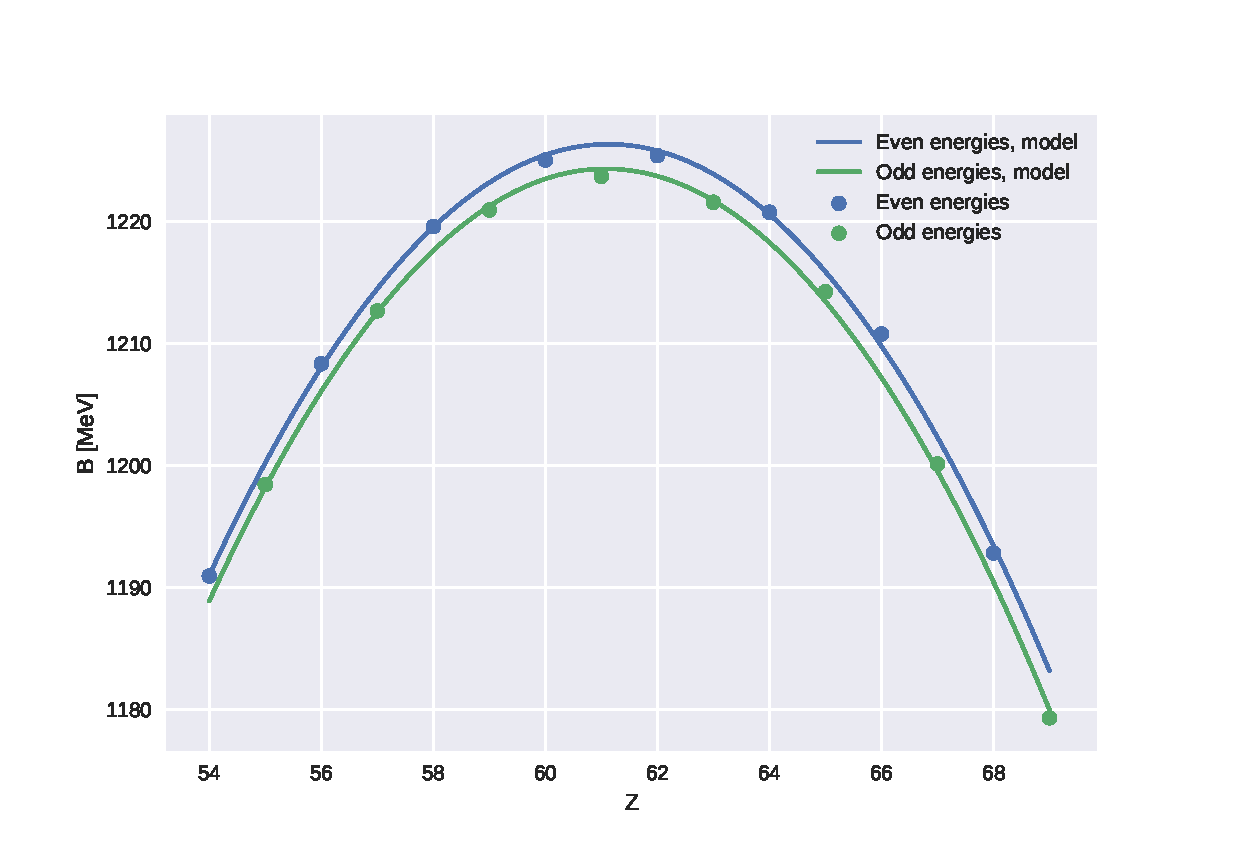
\includegraphics[width=\textwidth]{figures/parabolic_fits.eps}
      \caption{Fit and raw data}
  \end{subfigure}%
  \begin{subfigure}{0.5\textwidth}
      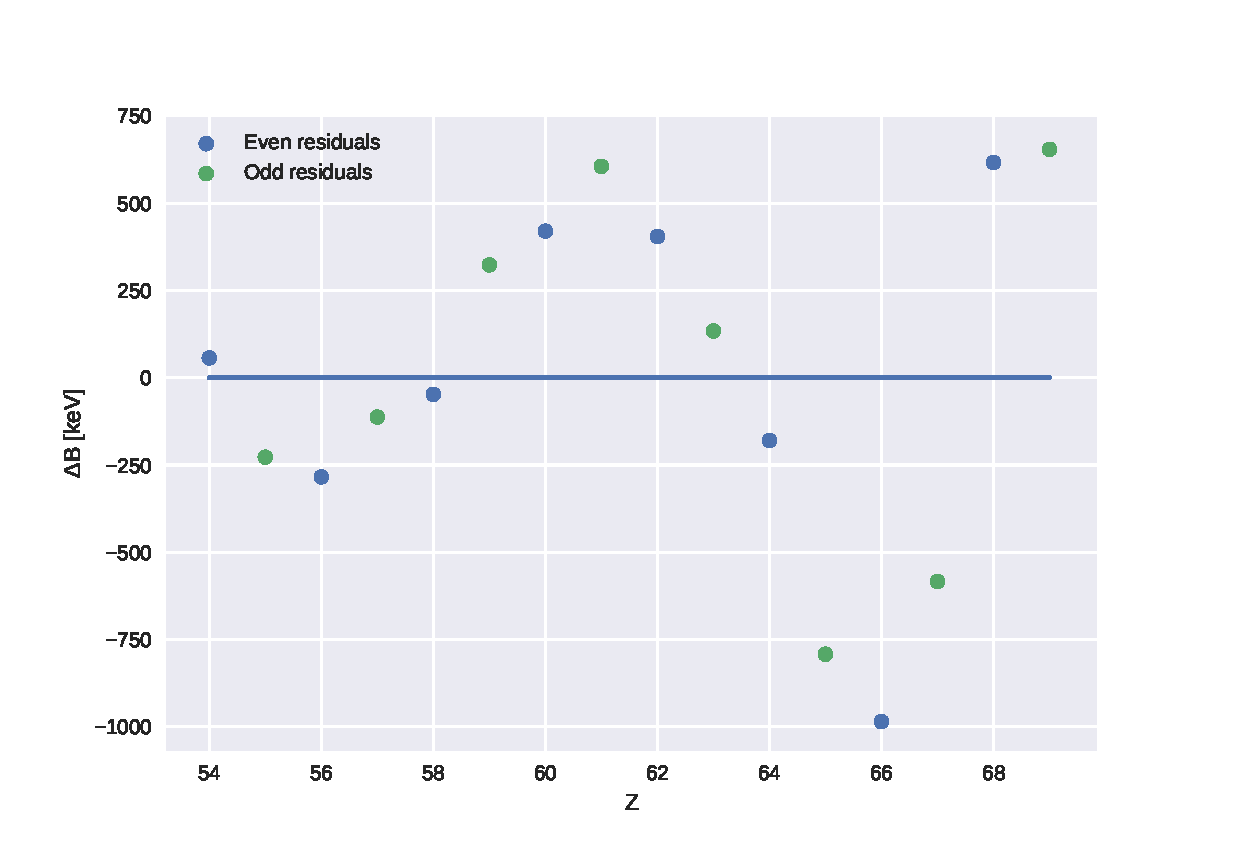
\includegraphics[width=\textwidth]{figures/residuals.eps}
      \caption{Residuals of the fit}
  \end{subfigure}
  \caption{Mass parabola fit}
  \label{fig:mass-parabola-fit}
\end{figure}

There are some odd-odd stable nuclei, like \(^{14} \ce{N} \), but they are rare.

\paragraph{Specular nuclei}

If they have \(\Delta Z = 1\) and \(A\) is odd, interesting things happen. Our working example is \(^{15} _{8   } \ce{O} _{7} \) and \(^{15} _{7} \ce{N}_8 \).

The only term which changes in the SEMF between them is the Coulomb term: their \(Z\)s are \((A \pm 1)/2\), therefore (applying the corrected Coulomb formula given in \eqref{eq:SEMF-coulomb-correction}) their difference in energy is given by

\begin{subequations}
\begin{align}
  \Delta B  &= \frac{a_C}{A^{1/3}} \qty(\frac{(A+1)(A-1)}{4} - \frac{(A-1)(A-3)}{4})  \\
  &= \frac{a_C}{A^{1/3}} \qty(\frac{4A -4}{4})  \\
  &= a_C \qty(A^{2/3} - A^{-1/3})
\end{align}
\end{subequations}

We can plot the data for \(\Delta B\) wrt \(x \defeq A^{2/3}\). The plot will be of the form

\begin{equation}
    \Delta B  = a_C x - \frac{a_C}{\sqrt{x}}
\end{equation}

The fit works, giving us \(a_C = \SI{631(5)}{keV}\) in this parametrization.

\begin{figure}[H]
    \centering
    \begin{subfigure}{0.5\textwidth}
        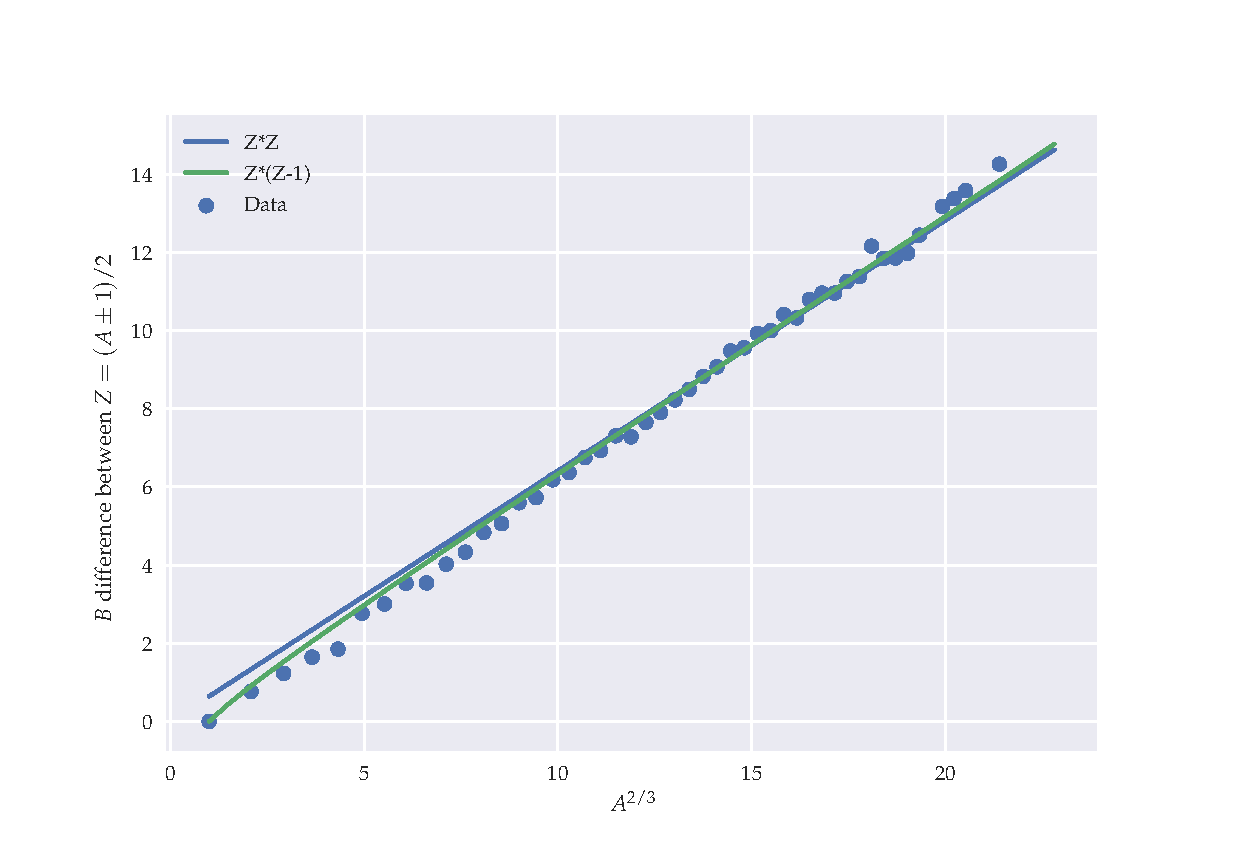
\includegraphics[width=\textwidth]{figures/odd_A_fit.eps}
        \caption{Fit}
    \end{subfigure}%
    \begin{subfigure}{0.5\textwidth}
        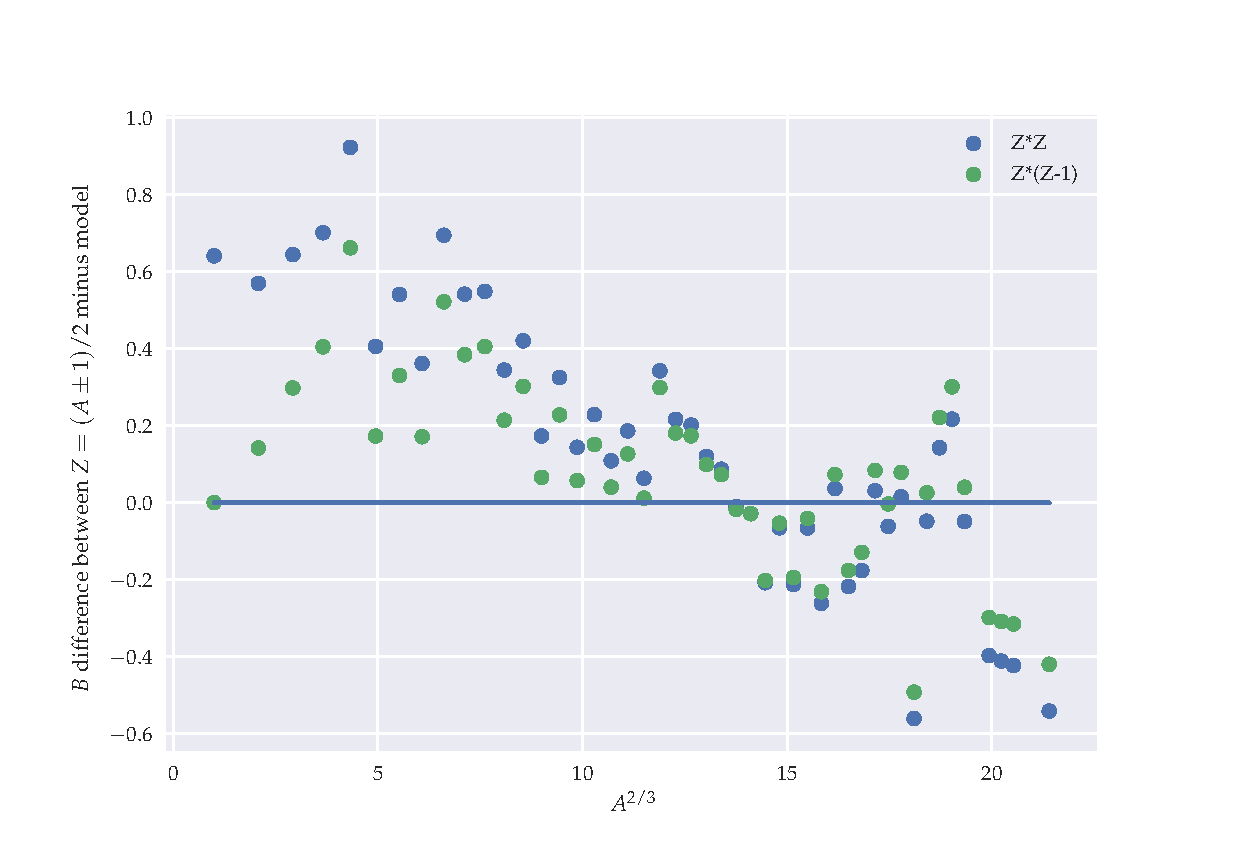
\includegraphics[width=\textwidth]{figures/odd_A_residuals.eps}
        \caption{Residuals}
    \end{subfigure}%
    \caption{Fit of the difference in \(B\) between symmetric nuclei. The chi square is \(\SI{0.136}{MeV^2} \) for the \(Z^2\) model, and \(\SI{0.062}{MeV^2}\) for the \(Z(Z-1)\) model.}
    \label{fig:odd-A-fit}
\end{figure}

\section{Fermi gas model}

\paragraph{Hypotheses}

\begin{itemize}
    \item The nucleons are spin \(1/2\) fermions;
    \item the nucleons' collective actions can be represented with a spherically symmetric potential well \(U(r)\), extended in a radius \(R = r_0 A^{1/3}\);
    \item the nucleon gas is degenerate: the kinetic energy of the nucleons is much less than the thermal energy \(k_B T\).
\end{itemize}

The proper Hamiltonian, without the mean-field approximation,  would be

\begin{equation}
    H = \sum _{i} T_i + \sum _{i<j} V_{ij} \qty(\abs{r_i - r_j} )
\end{equation}

instead, we use

\begin{equation}
    H_{\text{sp}} = -\frac{\hbar^2 \nabla^2}{2 \mu} + U(r)
\end{equation}

where \(\text{sp}\) means 'single particle', \(\mu ^{-1} = m _{\text{sp}} ^{-1} + m _{\text{nucleus}} ^{-1}\).

For nuclei at human temperatures, \(\lesssim \SI{e3}{K} \), we have energies \(\lesssim \frac{3}{2} k_B T = \SI{0.13}{eV}  \ll MeV \), so thermal motion is negligible.

\paragraph{\(1D\) infinite well}

We have an infinite well from \(-a/2\) to \(a/2\), and inside it a particle of mass \(m\).

The solutions to the time-independent Schrödinger equation are in the form

\begin{equation}
    \psi(x) = A \sin(kx) +B \cos(kx)
\end{equation}

where \(k^2  = 2mE / \hbar^2\) is the square of the wavenumber, which is directly proportional to the momentum \(k = p/\hbar = 2 \pi / \lambda\). We must also consider the boundary conditions: the domain of the Hamiltonian is \(\qty{\psi(x) \in L^2 \,|\, \psi(\pm a/2)=0 } \).

So we have two classes of solutions, proportional to either \(\cos((2q)\pi x/a)\) or \(\sin((2q+1)\pi x/a)\) with \(n
\in \N\). If we call the even or odd number \(2q (+1) = n_x\), the energy comes out to be

\begin{equation}
    E = \frac{\hbar^2 k^2}{2m} = \frac{h^2 n_x^2}{8ma^2}
\end{equation}

\paragraph{\(3D\) potential well}

The problem works out analogously, with

\begin{equation}
    E = \frac{h^2}{8ma^2} \sum _i  n_i^2
\end{equation}

so we work in the space \(\Z_+^3 \ni \vec{n} \), where same-energy states live in spherical shells.

The differential number of states in these shells is (approximately) given by the volume of the shell, which is an eighth of the sphere's: \(N = \frac{1}{8} 4 \pi n^2 \dd{n} \). This can also be written as \(\rho(E) \dd{E} \), that is, it corresponds to a density of states.

Then, since the energy is just a function of \(n\), we have

\begin{equation}
    \dd{E} = \frac{h^2}{8ma^2} \dd{(n^2)} =   \frac{h^2}{4ma^2} n\dd{n}
\end{equation}

Therefore we can substitute in:

\begin{equation}
    \rho(E) \dd{E} = \frac{\pi}{2} \underbrace{n}_{\substack{\sqrt{8ma^2 E/h^2}}} \underbrace{n \dd{n} }_{\substack{4ma^2 / h^2} \dd{E} } = \frac{2 \pi  \qty(2ma^2)^{3/2}}{h^3} \sqrt{E} \dd{E}
\end{equation}

and we can also express this wrt \(p = \sqrt{2mE} \); its differential is \(p\dd{p} = m \dd{E} \):

\begin{equation}
    \rho(p) \dd{p} = V \frac{4 \pi a^3 p^2 \dd{p} }{h^3} 
\end{equation}

\end{document}
